\documentclass[journal]{IEEEtran}

\usepackage{amsmath,amssymb,amsfonts}
\usepackage{graphicx}
\usepackage{textcomp}
\usepackage{xcolor}
\usepackage{booktabs}
\usepackage{multirow}
\usepackage{url}
\usepackage{float}
\usepackage{cite}
\usepackage{mdframed}
\usepackage{tikz}
\usepackage{pgfplots}
\usetikzlibrary{arrows.meta,positioning,shapes.geometric,fit,calc,backgrounds}
\pgfplotsset{compat=1.18}
\usepackage{hyperref}

% ── Color definitions (Rule Q) ──────────────────────────────────────────────
\definecolor{darkblue}{RGB}{0,0,139}
\definecolor{midgreen}{RGB}{34,139,34}
\definecolor{deepred}{RGB}{180,0,0}
\definecolor{steelblue}{RGB}{52,102,153}
\definecolor{tealcolor}{RGB}{0,110,110}
\definecolor{ambercolor}{RGB}{204,102,0}
\definecolor{slateblue}{RGB}{90,80,160}

% ── Suppress IEEEtran's hardcoded Abstract/Keywords labels ──────────────────
\makeatletter
\def\abstract{\normalfont
    \if@twocolumn
      \relax
    \else
      \bgroup\par\addvspace{0.5\baselineskip}\centering\vspace{-1.78ex}%
      \@IEEEabskeysecsize\textbf{\abstractname}%
      \par\addvspace{0.5\baselineskip}\egroup\quotation\@IEEEabskeysecsize
    \fi\@IEEEgobbleleadPARNLSP}
\def\IEEEkeywords{\normalfont
    \if@twocolumn
      \relax
    \else
      \bgroup\par\addvspace{0.5\baselineskip}\centering\@IEEEabskeysecsize%
      \textbf{\IEEEkeywordsname}%
      \par\addvspace{0.5\baselineskip}\egroup\quotation\@IEEEabskeysecsize
    \fi\@IEEEgobbleleadPARNLSP}
\makeatother

\begin{document}

\title{\textcolor{darkblue}{Forward Deployed Engineer (FDE) in the AI Ecosystem}}

\author{%
  \IEEEauthorblockN{\textcolor{slateblue}{\itshape Muhammad Faisal Laiq
    \qquad Email:~shmlaiq@gmail.com \qquad
    ORCID:~0009-0007-5779-9836}}%
}

\maketitle

\begin{abstract}
\begin{mdframed}[
  linecolor=darkblue, linewidth=1.8pt,
  backgroundcolor=darkblue!5,
  innerleftmargin=10pt, innerrightmargin=10pt,
  innertopmargin=9pt, innerbottommargin=9pt,
  roundcorner=5pt, skipabove=0pt, skipbelow=0pt
]
\noindent\textbf{\textcolor{darkblue}{Abstract\,---}}~``Forward Deployed Engineer'' (FDE) job postings multiplied across AI companies between 2023 and 2025, but the title has no shared definition --- teams confuse it with Solutions Architect, Sales Engineer, and plain Software Engineer, then staff and pay it like one of those roles instead of what it actually is. This article proposes a six-dimension way to tell FDE apart from four adjacent roles, a competency profile built from real hiring evidence, and a four-stage engagement lifecycle with the feedback loop most teams don't budget for. It compares how Palantir, OpenAI, Anthropic, and Scale AI run their FDE programs from public sources, and closes with three concrete actions engineering leaders can take this quarter --- before the next FDE requisition gets written from a Solutions Architect template.
\end{mdframed}
\end{abstract}

\begin{IEEEkeywords}
\begin{mdframed}[
  linecolor=darkblue!35, linewidth=0.8pt,
  backgroundcolor=darkblue!3,
  innerleftmargin=8pt, innerrightmargin=8pt,
  innertopmargin=5pt, innerbottommargin=5pt,
  roundcorner=3pt, skipabove=0pt, skipbelow=4pt
]
\noindent\textbf{\textcolor{darkblue}{Index Terms\,---\,}}Forward deployed engineering, enterprise AI deployment, engineering roles, hiring practice
\end{mdframed}
\end{IEEEkeywords}

\vspace{4pt}
\begin{mdframed}[
  linecolor=midgreen, linewidth=1.6pt,
  backgroundcolor=midgreen!6,
  innerleftmargin=10pt, innerrightmargin=10pt,
  innertopmargin=8pt, innerbottommargin=8pt,
  roundcorner=5pt
]
\noindent\textbf{\textcolor{midgreen}{Three Actionable Insights}}
\begin{itemize}
  \item \textbf{Stop hiring FDEs against a Solutions Architect job description.} Ambiguity tolerance --- not client-facing hours --- is the trait that actually separates the two roles. Screen for it directly: give candidates an underspecified problem, not a system-design exercise.
  \item \textbf{Budget every FDE engagement for a return trip to discovery.} Teams that plan Discovery~$\to$~Prototype~$\to$~Integration~$\to$~Handoff as four fixed-length phases consistently blow their timeline, because Integration routinely surfaces constraints Discovery couldn't have found.
  \item \textbf{Write down your handoff plan before the engagement starts, not after.} The single most common FDE program failure isn't a bad deployment --- it's a good one nobody owns six months later.
\end{itemize}
\end{mdframed}
\vspace{4pt}

\section{Introduction}
\label{sec:intro}

\IEEEPARstart{J}{ob} postings for ``Forward Deployed Engineer'' multiplied across AI-native companies between 2023 and 2025. By the time OpenAI stood up a dedicated FDE function in 2025, forward-deployed and solutions-engineering roles already accounted for 22 of the company's 311 open positions \cite{schmidt2025servicesledgrowth}. Palantir popularized the title over a decade earlier --- engineers embedded directly with clients, internally called ``Delta,'' building and modifying software against operational needs that shifted week to week; for several years before 2016, Palantir employed more FDEs than conventional software engineers \cite{orosz2025fde}. What changed since 2023 is scale and imitation: OpenAI, Anthropic, and Scale AI have each stood up teams under the same label or a close variant \cite{openai2026fdelifesciences,anthropic2026fde,scaleai2026fde}.

No engineering body defines it. A Solutions Architect also goes to the client. So does a Site Reliability Engineer (SRE) doing an onsite incident postmortem. That gloss --- ``an engineer who goes to the client'' --- collapses distinctions that matter the moment you try to hire, level, or pay for the role. Recruiters copy Solutions Architect job descriptions and add ``willingness to travel.'' Compensation teams benchmark FDE pay against sales scales never designed for engineers who ship production code. Engineering leaders staff FDE teams with generalist engineers who lack client-facing training, then wonder why every engagement stalls in discovery.

The closest precedent for what happens next is Site Reliability Engineering. SRE existed as an internal Google practice for years --- a hybrid discipline everyone recognized but nobody had formally written down --- before Google's own account of the practice turned it into a hireable, teachable, industry-wide discipline \cite{beyer2016sre}. FDE is at roughly that pre-codification stage today. This article is an attempt to do that codification step early enough to shape hiring practice, not just describe it after the fact.

Large language model (LLM) deployment inside enterprises makes the stakes concrete: a systematic review of 63 enterprise retrieval-augmented generation (RAG) and LLM adoption studies found fewer than 15\% addressed the real-time integration challenges production deployment actually requires \cite{karakurt2026rag}. That gap --- between what a model demonstrates in a benchmark and what it takes to make it work on one company's real data --- is exactly the terrain FDEs are hired to cover, and exactly what a Solutions Architect job description was never built to screen for.

\section{What an FDE Actually Is}
\label{sec:whatisfde}

An FDE is an engineer with full authority to modify a vendor's product --- not merely configure it --- embedded inside a specific client's environment to close the gap between a horizontal AI product and that client's operational workflow, under open-ended technical and organizational ambiguity. Three clauses do the real work. \emph{Full authority to modify the product} excludes Solutions Architects, who design against existing extension points rather than change core code. \emph{Embedded inside a specific client's environment} excludes ML Research Engineers, whose audience is the model or the research community, not a paying account. \emph{Open-ended ambiguity} excludes conventional Software Engineers working a backlog a product manager has already scoped for them.

Table~\ref{tab:matrix} lays out the distinction that actually matters for hiring: ambiguity tolerance, not client-interaction frequency. A Sales Engineer talks to clients constantly too, but under a bounded question --- does the product meet the stated requirement, yes or no. An FDE routinely doesn't know, at the start of an engagement, whether the requirement is solvable with the current product at all. That's the job. Hiring bars and comp bands built around ``client-facing hours'' alone will consistently mis-level this role against Sales Engineering, understating the technical bar it actually requires.

\begin{table*}[t]
\caption{FDE vs.\ Four Adjacent Roles}
\label{tab:matrix}
\centering
\footnotesize
\begin{tabular}{p{2.1cm}p{3.4cm}p{2.9cm}p{3.4cm}p{3.4cm}}
\toprule
\textbf{Dimension} & \textbf{FDE} & \textbf{SWE} & \textbf{ML Research Engineer} & \textbf{Solutions Architect} \\
\midrule
Primary output & Working integration in client's stack & Shipped product feature & Model/experiment artifact & Design recommendation \\
Client interaction & Continuous, embedded & Rare, mediated & Minimal & High, pre-sale/advisory \\
Ambiguity tolerance & Very high --- undefined problem AND solution & Low --- scoped tickets & High on research, low on audience & Moderate --- defined ask \\
Travel expectation & High (one company quantifies at 25\% \cite{anthropic2026fde}) & Low & Low & Moderate \\
\bottomrule
\end{tabular}
\end{table*}

\section{What Makes a Good FDE}
\label{sec:competency}

Two competencies dominate, and neither shows up in a standard technical interview. The first is integration engineering against unfamiliar, undocumented client systems under time pressure --- legacy databases, internal APIs, formats nobody wrote down --- plus the AI-specific version of that skill: debugging why a RAG pipeline degrades silently on one client's real document corpus, or why an agent's behavior, reliable in evaluation, breaks on a query pattern the benchmark never saw \cite{karakurt2026rag,mohammadi2025llmagentsurvey,brehme2025ragtrust}. The second is discovery facilitation --- running a working session that extracts a client's actual operational problem when the client hasn't fully articulated it themselves. It's arguably the single most valuable FDE skill, and it's almost never assessed in a hiring loop built for engineers.

Fig.~\ref{fig:lifecycle} shows why the engagement itself resists the flat, phase-by-phase project plan most teams default to. Discovery narrows scope to something achievable; Prototype routinely reveals the narrowed scope was still wrong, because a client's stated workflow and their actual workflow diverge in ways nobody notices until code runs against real data. That divergence forces a return to Discovery --- the dashed loop in the figure --- and teams that budget four fixed-length sequential phases consistently underrun their timeline because they never planned for that loop.

\begin{figure*}[t]
\centering
\resizebox{0.96\textwidth}{!}{%
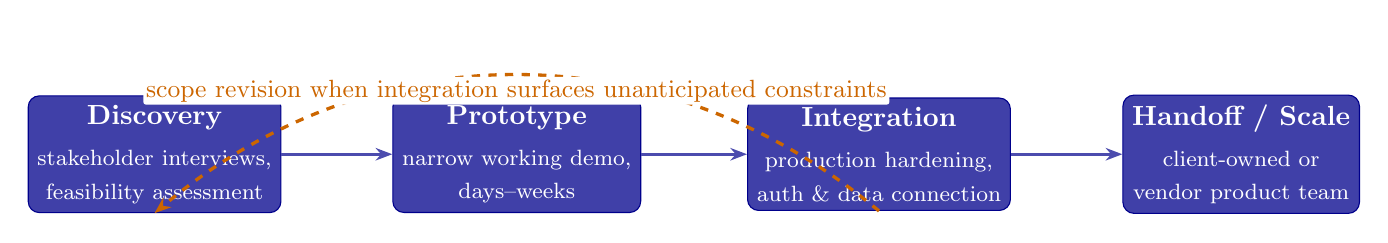
\begin{tikzpicture}[
  proc/.style={rectangle,rounded corners=4pt,draw=darkblue,fill=darkblue!75,
               text=white,minimum width=3.0cm,minimum height=1.3cm,align=center,
               font=\normalsize\bfseries},
  ar/.style={-{Stealth[length=6pt]},very thick,darkblue!70},
  fb/.style={-{Stealth[length=6pt]},very thick,ambercolor,dashed},
  lab/.style={font=\small,fill=white,inner sep=1pt,rounded corners=1pt}
]
\node[proc] (disc) at (0,0)    {Discovery\\[3pt]\footnotesize\normalfont stakeholder interviews,\\\footnotesize\normalfont feasibility assessment};
\node[proc] (prot) at (4.6,0)  {Prototype\\[3pt]\footnotesize\normalfont narrow working demo,\\\footnotesize\normalfont days--weeks};
\node[proc] (integ) at (9.2,0) {Integration\\[3pt]\footnotesize\normalfont production hardening,\\\footnotesize\normalfont auth \& data connection};
\node[proc] (hand) at (13.8,0) {Handoff / Scale\\[3pt]\footnotesize\normalfont client-owned or\\\footnotesize\normalfont vendor product team};

\draw[ar] (disc) -- (prot);
\draw[ar] (prot) -- (integ);
\draw[ar] (integ) -- (hand);

\draw[fb] (integ.south) to[bend right=40]
  node[lab,below,pos=0.5]{scope revision when integration surfaces unanticipated constraints} (disc.south);
\end{tikzpicture}%
}
\caption{The FDE engagement lifecycle. Discovery, Prototype, Integration, and Handoff/Scale form the main sequence (solid arrows); the dashed feedback arrow denotes the common case in which integration-stage findings force a return to Discovery.}
\label{fig:lifecycle}
\end{figure*}

The Handoff/Scale stage has its own quiet failure mode, and it's organizational, not technical: client teams frequently lack the capacity to maintain what the FDE built, leaving the vendor holding informal, unstaffed maintenance responsibility for code nobody budgeted as a long-term product. Anthropic's own FDE role description names this directly --- ``identify and codify repeatable deployment patterns'' is a partial, informal answer to it, not a solved one \cite{anthropic2026fde}.

\section{How Four AI Companies Are Doing It}
\label{sec:cases}

Palantir remains the reference implementation: FDE as a first-class engineering discipline with a documented pipeline into product roles, not a support function bolted onto sales \cite{orosz2025fde,palantir2026fdse}. OpenAI's version is younger and unusually well-documented for its age --- Colin Jarvis built the business case in early 2025, the team grew from two FDEs to more than ten across eight cities on three continents, and OpenAI draws the Solutions-Architect boundary explicitly: Solutions Architects advise, FDEs write code directly on customer infrastructure under real ambiguity \cite{orosz2025fde}. Anthropic runs FDE inside its Applied AI team with unusual specificity in its own posting --- deliverables named as ``MCP servers, sub-agents, and agent skills,'' travel quantified at 25\%, four-plus years of customer-facing experience required \cite{anthropic2026fde}. Scale AI's solutions and deployment function grew out of data-labeling and evaluation infrastructure rather than a general-purpose product needing client adaptation --- a different starting point than the other three, even where the resulting job title looks the same on a careers page --- a characterization this analysis holds with less confidence than the other three, given limited independent verification of the current posting \cite{scaleai2026fde}.

The clearest pattern across all four isn't structural convergence so much as a documentation gap: Palantir's decade-plus public track record dwarfs the other three, largely because it has one and they don't yet. That's a disclosure asymmetry, not necessarily a maturity one --- this analysis can't tell ``less mature'' apart from ``less publicly documented'' from public sources alone. What's consistent regardless: all four give FDEs real product-modification authority inside a client's environment, all four treat that as distinct from conventional sales engineering, and none has published a formal competency framework of the kind this article proposes.

\section{Limitations and What's Next}
\label{sec:limitations}

This framework is descriptive, not causal --- it says what FDE work looks like across public job postings, not that any one dimension predicts a good engagement, because no engagement-outcome data was collected to test that. Every claim about the four named companies comes from public, often company-authored material that naturally emphasizes program strengths; take the case comparison with that discount in mind. And role titles at this boundary are multiplying fast --- ``Applied AI Engineer,'' ``AI Solutions Engineer'' --- so a taxonomy built from a 2026 snapshot will need revisiting inside two years, not five.

The next real step is a practitioner survey: score actual FDEs and their managers against these dimensions and against concrete engagement outcomes. Nothing in Section~\ref{sec:competency} has been tested against outcomes yet --- that's the honest gap, and it's the highest-priority one to close.

\section{Conclusion}
\label{sec:conclusion}

The FDE title is doing real organizational work right now without a definition to back it up. Section~\ref{sec:whatisfde}'s distinction --- ambiguity tolerance over client-interaction frequency --- is the one hiring managers most often get backwards. Section~\ref{sec:competency}'s lifecycle model gives engineering leaders a planning tool the flat sequential mental model doesn't provide. None of that requires waiting for a formal academic consensus to start using: the three actions at the top of this article are usable on the next FDE requisition your team writes.

\section*{Acknowledgment}
This work received no external funding or institutional support. All source material is drawn from publicly accessible company career pages, industry publications, and peer-reviewed literature, as cited throughout.

This article's text was drafted with the assistance of Claude (Anthropic), an artificial intelligence system, under the direction, review, and fact-verification of the author, who is fully accountable for all content, citations, and claims. No AI system is credited as an author.

\bibliographystyle{IEEEtran}
\bibliography{references}

\end{document}
